\documentclass[conference]{IEEEtran}

\usepackage{cite}
\usepackage{amsmath,amssymb}
\usepackage{graphicx}
\usepackage{booktabs}
\usepackage{array}
\usepackage{float}
\usepackage{balance}
\usepackage{url}
\usepackage[hidelinks]{hyperref}

\title{Budget-Constrained Vector-Graph Evidence Retrieval for Low-Latency Mechanical Fault Assistance with a Local 7B LLM}

\author{
\IEEEauthorblockN{Xiaokun Zhang\textsuperscript{1},
Dongliang Fu\textsuperscript{1}, and
Rui Wang\textsuperscript{2,*}}
\IEEEauthorblockA{\textsuperscript{1}Shanghai Marine Equipment Research Institute (SMERI), China State Shipbuilding Corporation (CSSC), Shanghai, China}
\IEEEauthorblockA{\textsuperscript{2}College of Electronic and Information Engineering, Tongji University, Shanghai 201804, China\\
\textsuperscript{*}Corresponding author: Rui Wang (\href{mailto:ruiwang@tongji.edu.cn}{ruiwang@tongji.edu.cn})}}

\begin{document}
\maketitle

\begin{abstract}
Deploying retrieval-augmented mechanical fault assistance with a local language model requires balancing evidence coverage against inference cost. Under a small evidence budget, dense top-$k$ retrieval may spend limited slots on task-misaligned, fault-mismatched, or redundant passages, thereby lengthening prompts and triggering unnecessary model calls. We present a budget-constrained vector-graph evidence retrieval method that converts broad BGE-M3 recall into at most three complementary evidence items. It combines diagnostic-task and fault-scope constraints, one-hop graph proximity, source-family novelty, and active underfilling. A fixed Qwen2.5-7B model performs only binary support verification, after which a deterministic renderer produces evidence-linked fault-assistance suggestions or abstains. On 40 marine pump fault queries, the complete method improves Recall from 0.218 to 0.431, NDCG from 0.406 to 0.822, and citation F1 from 0.259 to 0.426 over dense retrieval under the same maximum budget. It reduces mean prompt length by 40.5\%, model calls by 39.0\%, and end-to-end latency by 36.7\%. The system answers all 34 designated answerable queries and abstains on all six designated unanswerable queries. An automated same-model, dual-prompt audit finds that 91.0\% of atomic answer points are strictly supported by cited spans. These results show that retrieval-side evidence budgeting can improve grounding while reducing the inference workload of a fixed local model.
\end{abstract}

\begin{IEEEkeywords}
hybrid retrieval, graph retrieval, evidence budgeting, retrieval-augmented generation, mechanical fault diagnosis, local language model
\end{IEEEkeywords}

\section{Introduction}

Mechanical fault assistance in ship engine rooms must return useful symptom interpretations, possible causes, inspection steps, or maintenance actions within a short response time. Retrieval-augmented generation (RAG) can ground a language model in technical documents \cite{lewis2020rag}, but retrieving more text is not always beneficial. For a local 7B model, unrelated or repeated passages consume context and trigger additional evidence checks. Both effects increase latency, which is undesirable when the eventual system must operate under limited computing resources.

Dense retrievers provide broad semantic recall but do not reliably distinguish diagnostic roles such as symptom, cause, inspection, and maintenance. Graph-based retrieval can recover structurally related evidence \cite{edge2024graphrag,sun2024think,he2024gretriever,zhu2025kg2rag}; however, uncontrolled graph expansion can enlarge the same context that a small model must process. We therefore study a constrained question: with the model and maximum evidence count fixed, can vector relevance and local graph structure select fewer, more useful evidence items while improving answer support and reducing end-to-end latency?

Our contributions are as follows:
\begin{itemize}
    \item We formulate evidence selection as a budgeted hybrid retrieval problem. Dense similarity, diagnostic-role compatibility, fault affinity, one-hop graph proximity, and source novelty are combined under a hard maximum of three evidence items, with active underfilling when no qualified item remains.
    \item We couple the selector to a low-output local-model protocol: Qwen2.5-7B only returns binary support decisions, while a deterministic renderer creates cited answer points or an explicit abstention. This separation reduces prompt length, model calls, and unsupported free-form generation.
    \item We evaluate retrieval quality, citation accuracy, answer and abstention behavior, and CUDA-synchronized latency under equal evidence budgets. The results establish a quality-efficiency gain without changing or fine-tuning the local model.
\end{itemize}

\section{Related Work}

BGE-M3 supports multilingual, multi-function, and multi-granularity representations \cite{chen2024bgem3}, while Qwen2.5 provides open-weight instruction models at several scales \cite{yang2024qwen}. We fix Qwen2.5-7B throughout the study. Unlike prompt compressors that rewrite the context \cite{jiang2023llmlingua}, our method preserves verbatim evidence and reduces the amount selected before generation.

GraphRAG and related systems use graph search or retrieved subgraphs to guide generation \cite{edge2024graphrag,sun2024think,he2024gretriever,zhu2025kg2rag}. We use only one-hop propagation as a bounded retrieval signal, not open-ended path reasoning. ALCE \cite{gao2023alce} and RAGAs \cite{es2024ragas} motivate explicit evaluation of citation and faithfulness, while selective question answering \cite{kamath2020selective} and Self-RAG \cite{asai2024selfrag} show the value of abstention and self-checking. Our focus is the joint control of evidence quality and inference cost in a hybrid vector-graph pipeline.

\begin{figure*}[!t]
    \centering
    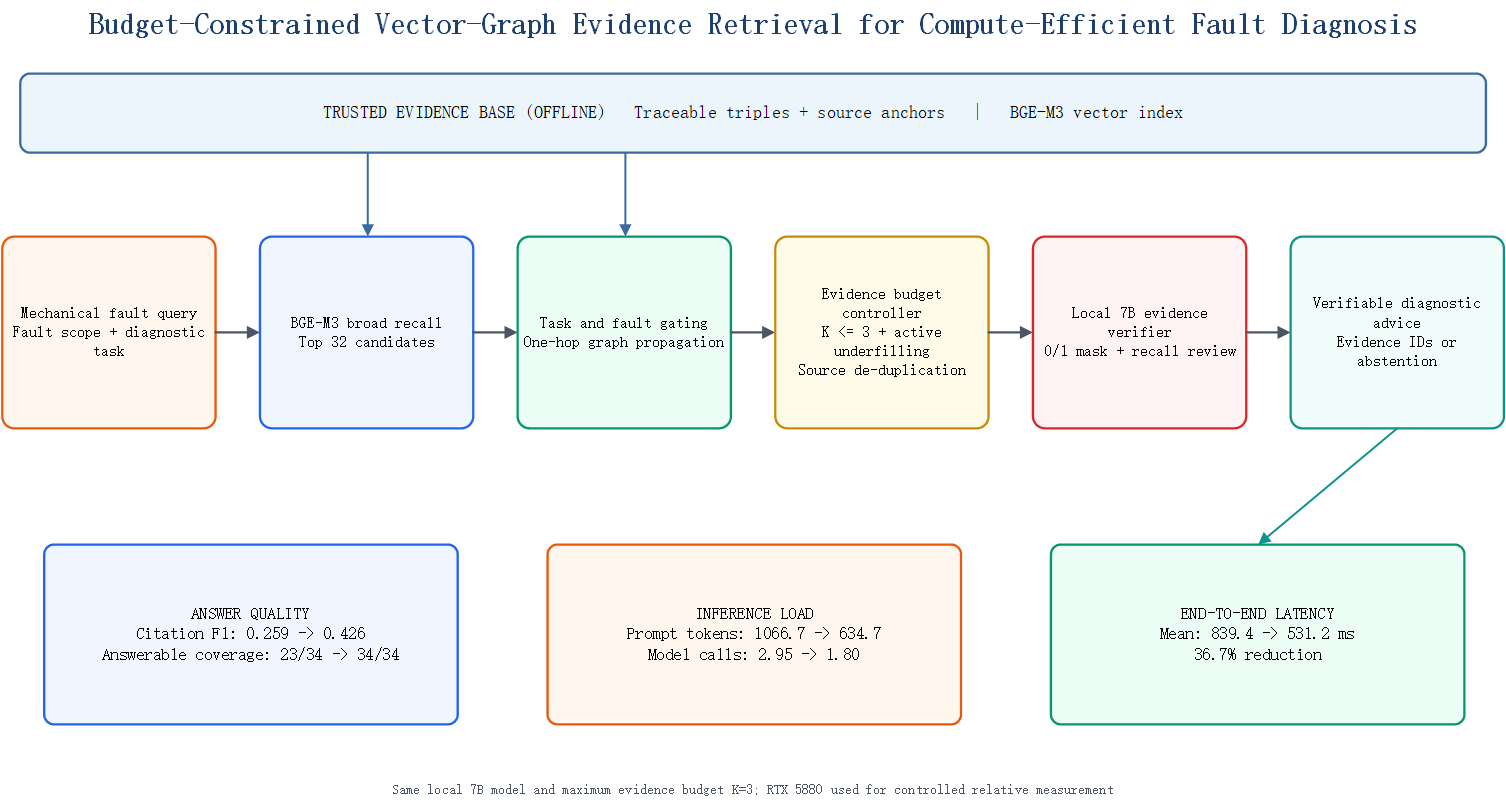
\includegraphics[width=0.98\textwidth]{figures/rp2_budgeted_retrieval_en.png}
    \caption{Budget-constrained vector-graph evidence retrieval. The online path narrows broad vector recall to a compact evidence set, asks the local 7B model only for support decisions, and returns evidence-linked suggestions or an explicit abstention.}
    \label{fig:pipeline}
\end{figure*}

\section{Budget-Constrained Vector-Graph Retrieval}

\subsection{Problem Formulation and Inference Load}

A query is represented as $q=(x,f,r)$, where $x$ is the natural-language question, $f$ is the specified fault scope, and $r$ is one of four diagnostic roles: symptom, cause or mechanism, inspection, and maintenance. Fault scope and role are structured system inputs; open-ended intent parsing is outside this study. A fixed offline evidence base supplies normalized triples, verbatim source spans, source identifiers, and BGE-M3 embeddings. Its construction is not a contribution of this paper.

For a local model, the online inference load is dominated by cumulative prompt tokens $T_{\mathrm{prompt}}$ and the number of model calls $N_{\mathrm{call}}$. We use
\begin{equation}
L_{\mathrm{inf}}(q)=\alpha T_{\mathrm{prompt}}(q)+\beta N_{\mathrm{call}}(q),
\label{eq:load}
\end{equation}
where $\alpha$ and $\beta$ depend on the hardware and inference stack. Rather than fitting these coefficients, we report prompt tokens, calls, and measured end-to-end latency separately. The evidence budget links retrieval quality to this inference load.

\subsection{Broad Recall, Graph Signal, and Budgeting}

BGE-M3 first returns the top 32 candidates. The endpoint entities of the top eight items become graph anchors, and their scores propagate for one hop with a decay of 0.70. The base score of evidence item $e$ is
\begin{equation}
b(e,q)=s_d(e,q)+0.24s_g(e,q)+0.10c(e)+0.35a(e,q),
\label{eq:base}
\end{equation}
where $s_d$ is dense similarity, $s_g$ is one-hop graph proximity, $c(e)$ is an evidence-confidence prior, and $a(e,q)$ is a character-bigram Dice affinity between the fault name and evidence endpoints. Role gating retains evidence that matches the requested diagnostic task, and fault gating removes visible scope mismatches.

Candidates are greedily selected by the marginal score
\begin{equation}
\Delta(e\mid S,q)=b(e,q)+0.06\,\mathbb{I}[\phi(e)\notin\Phi(S)],
\label{eq:select}
\end{equation}
where $\phi(e)$ denotes the source family. The novelty term discourages repeated evidence from the same organization or manual family. Selection satisfies $|S|\leq K$, with $K=3$. The budget is a ceiling, not a target: the selector stops when remaining candidates violate the role or fault constraints.

\subsection{Binary Verification and Deterministic Answers}

Qwen2.5-7B does not freely compose the diagnostic response. In stage 1, it returns one binary support decision for each selected evidence item. Stage 2 independently rechecks only rejected candidates with a recall-oriented prompt, again returning a single 0 or 1. Invalid JSON, length mismatches, or nonbinary outputs are treated as unsupported. A deterministic renderer converts accepted evidence into atomic answer points with evidence identifiers. If none remains, the system reports insufficient evidence.

Figure \ref{fig:pipeline} summarizes the workflow. For example, on a pump-motor misalignment cause query, the complete selector returned three complementary assertions. The local verifier produced the mask $[1,1,1]$, and the renderer reported excessive coupling wear, pump vibration, and premature bearing failure as separate cited points. The example illustrates why the model is used as a verifier rather than as an unconstrained technical author.

\section{Experimental Design}

\subsection{Benchmark and Equal-Budget Baselines}

The benchmark contains 40 queries spanning ten pump-fault classes and four diagnostic roles: 34 are answerable and six test abstention. The online store contains 208 evidence assertions from 14 documents in ten source families; relevance labels are hidden from every online method. Two deterministic paraphrases per query yield 80 untuned robustness queries. Seven answerable queries from an isolated external set provide a post-freeze, no-feedback check and are not used for statistical inference.

All methods share the maximum budget $K=3$. \emph{Dense} uses BGE-M3 similarity; \emph{Role} adds diagnostic-role gating; \emph{Role+Graph} adds one-hop propagation; and \emph{Full} adds fault affinity, source novelty, active underfilling, and two-stage verification. \emph{Full-NoGraph} disables only graph propagation.

\subsection{Metrics and Runtime Protocol}

We report Recall and NDCG for retrieval; citation precision, recall, and F1; answerable-query recall; abstention recall; and strict atomic support. Citation precision, recall, and F1 are macro-averaged independently over answerable queries, so F1 is not recomputed from aggregate precision and recall. Efficiency metrics are prompt tokens, model calls, stage latency, and end-to-end latency. Confidence intervals use 5,000 paired bootstrap samples clustered by fault class.

Experiments ran on one 48-GB NVIDIA RTX 5880 Ada GPU. Qwen2.5-7B was loaded in BF16 without CPU or disk offload. Three interleaved method orders were measured per query with CUDA synchronization; quality uses one prespecified run and timing the per-query median. Latency includes retrieval, prompt construction, verification, and rendering, but excludes loading, indexing, and warm-up. Results therefore compare relative online cost on identical hardware rather than absolute embedded-device performance.

\section{Results}

\subsection{Answer Quality and End-to-End Efficiency}

\begin{table}[H]
\centering
\caption{Equal-budget results with maximum $K=3$}
\label{tab:main}
\setlength{\tabcolsep}{2.4pt}
\resizebox{\columnwidth}{!}{%
\begin{tabular}{lccccc}
\toprule
Method & Recall & NDCG & Citation P/R/F1 & Ans./Abs. R & Mean/p95 (ms) \\
\midrule
Dense & 0.218 & 0.406 & 0.574/0.197/0.259 & 0.676/1.000 & 839.4/1113.1 \\
Role & 0.378 & 0.678 & 0.721/0.299/0.372 & 0.853/1.000 & 782.1/1109.6 \\
Role+Graph & 0.405 & 0.716 & 0.750/0.302/0.377 & 0.882/1.000 & 805.5/1101.6 \\
\textbf{Full} & \textbf{0.431} & \textbf{0.822} & \textbf{0.799/0.370/0.426} & \textbf{1.000/1.000} & \textbf{531.2/892.5} \\
\bottomrule
\end{tabular}}
\end{table}

Table \ref{tab:main} reports the equal-budget results. Relative to Dense, Full improves Recall by 0.2127, NDCG by 0.4166, and citation F1 by 0.1672, while reducing mean end-to-end latency by 308.2 ms. The clustered 95 percent CIs are $[0.1496,0.2748]$, $[0.3184,0.4940]$, $[0.1075,0.2298]$, and $[-395.3,-217.2]$ ms, respectively. None crosses zero. The quality gain therefore does not depend on a larger evidence input.

Full selects 2.25 evidence items on average. Mean prompt length falls from 1066.7 to 634.7 tokens, model calls from 2.95 to 1.80, and mean end-to-end latency from 839.4 to 531.2 ms, reductions of 40.5, 39.0, and 36.7 percent. The model is unchanged, so the savings arise from budgeted selection and active underfilling. In a separate synchronized breakdown, retrieval and prompt construction take 29.4 and 1.5 ms, model inference 504.1 ms, and deterministic rendering 0.07 ms; model inference remains the dominant cost.

\subsection{Attribution, Verification, and Evidence Support}

At the retrieval layer, adding one-hop propagation to Role increases Recall by 0.0268 (95 percent CI $[0.0031,0.0616]$) and NDCG by 0.0381 (95 percent CI $[0.0059,0.0804]$). In the complete system, Full and Full-NoGraph have similar means: Recall is 0.431 versus 0.429, NDCG 0.822 versus 0.800, and citation F1 0.426 versus 0.423. These mean differences are not significant. The graph signal nevertheless recovers one misalignment inspection query missed without it, raising answerable coverage from 33/34 to 34/34 at a 14.2 ms mean latency cost in the synchronized attribution run. We therefore interpret one-hop propagation as a low-cost tail-recall mechanism, not as the sole source of the system gain.

The two-stage verifier trades a small amount of precision for complete coverage. Stage 1 alone reaches 0.818 citation precision but misses one answerable query. Recall-oriented rechecking raises coverage to 34/34 while retaining 0.799 precision; all six unanswerable queries are rejected. An automated same-model, dual-prompt consistency audit covers 160 query-method outputs and 323 judged items, including 207 atomic answer points and 116 answer-level summaries. For Full, 91.0 percent of atomic answer points are strictly supported by cited source spans, 88.2 percent of answered responses have all atomic claims supported, and source-span verification is 100 percent. These are evidence-support measures, not expert-certified repair accuracy.

\subsection{Paraphrase Stability}

On 80 paraphrases excluded from parameter selection, Full obtains 0.383 Recall and 0.737 NDCG, compared with 0.338 and 0.645 for Role+Graph. The selected evidence has a mean Jaccard similarity of 0.742 with the parent queries, and the top-ranked item agrees in 72.5 percent of cases. The gain is therefore not tied to one fixed wording, although the fault scope and diagnostic role remain structured inputs.

\section{Discussion}

The practical contribution is a retrieval-side resource controller for local fault assistance. Dense recall protects candidate coverage; role and fault constraints remove mismatched evidence; one-hop propagation recovers structurally related tail items; and source novelty plus underfilling bounds the actual context. The 7B model performs only support classification, while deterministic rendering prevents new unsupported statements. This division of labor improves evidence-grounded responses and reduces the work assigned to the most expensive online component.

\balance
The design also matches a broader data-systems problem addressed by D2AI: coordinating vector and graph access paths under an explicit downstream budget. The offline graph is only a fixed input in this paper. Its source spans and identifiers make final suggestions inspectable, but graph construction is not claimed as a contribution here.

Two limitations define the current scope. First, the 40-query benchmark is a controlled capability test and provides the fault scope and diagnostic role; open-ended intent recognition remains future work. Second, relative latency was measured on a server GPU rather than on shipboard low-power hardware. A deployment study should keep the frozen model and retrieval policy while measuring memory, energy, concurrency, and absolute latency on the target platform.

\section{Conclusion}

This paper presented budget-constrained vector-graph evidence retrieval for compute-efficient mechanical fault assistance. Under a maximum of three evidence items, the method jointly uses dense relevance, task and fault constraints, local graph structure, and source diversity. Active underfilling and binary verification reduce unnecessary local-model inference. Within the evaluated marine-pump domain, the method improves retrieval and citation quality, shortens prompts, reduces model calls and end-to-end latency, and returns evidence-linked suggestions or a reliable abstention without increasing model size.

\section*{Declarations}
\textbf{Data availability:} Frozen configurations, code, derived evaluation records, and aggregate results will be released in a public repository. Copyrighted source PDFs are not redistributed. \textbf{Ethics and conflicts:} This study involves no human participants, animals, or personal data. The authors declare no known conflict of interest. \textbf{AI assistance:} Generative AI assisted code development, experiment-log organization, and language editing. The authors verified the study design, experiments, statistics, citations, and final manuscript.

\begin{thebibliography}{00}

\bibitem{lewis2020rag} P. Lewis et al., ``Retrieval-augmented generation for knowledge-intensive NLP tasks,'' in \emph{Advances in Neural Information Processing Systems}, vol. 33, pp. 9459--9474, 2020.

\bibitem{edge2024graphrag} D. Edge et al., ``From local to global: A graph RAG approach to query-focused summarization,'' arXiv:2404.16130, 2024, doi: 10.48550/arXiv.2404.16130.

\bibitem{chen2024bgem3} J. Chen, S. Xiao, P. Zhang, K. Luo, D. Lian, and Z. Liu, ``M3-Embedding: Multi-linguality, multi-functionality, multi-granularity text embeddings through self-knowledge distillation,'' in \emph{Findings of ACL 2024}, pp. 2318--2335, 2024, doi: 10.18653/v1/2024.findings-acl.137.

\bibitem{yang2024qwen} A. Yang et al., ``Qwen2.5 technical report,'' arXiv:2412.15115, 2024, doi: 10.48550/arXiv.2412.15115.

\bibitem{sun2024think} J. Sun et al., ``Think-on-Graph: Deep and responsible reasoning of large language model on knowledge graph,'' in \emph{Proc. ICLR}, 2024.

\bibitem{he2024gretriever} X. He et al., ``G-Retriever: Retrieval-augmented generation for textual graph understanding and question answering,'' in \emph{Advances in Neural Information Processing Systems}, vol. 37, pp. 132876--132907, 2024, doi: 10.52202/079017-4224.

\bibitem{zhu2025kg2rag} X. Zhu, Y. Xie, Y. Liu, Y. Li, and W. Hu, ``Knowledge graph-guided retrieval augmented generation,'' in \emph{Proc. NAACL-HLT}, vol. 1, pp. 8912--8924, 2025, doi: 10.18653/v1/2025.naacl-long.449.

\bibitem{gao2023alce} T. Gao, H. Yen, J. Yu, and D. Chen, ``Enabling large language models to generate text with citations,'' in \emph{Proc. EMNLP}, pp. 6465--6488, 2023, doi: 10.18653/v1/2023.emnlp-main.398.

\bibitem{es2024ragas} S. Es, J. James, L. Espinosa Anke, and S. Schockaert, ``RAGAs: Automated evaluation of retrieval augmented generation,'' in \emph{Proc. EACL System Demonstrations}, pp. 150--158, 2024, doi: 10.18653/v1/2024.eacl-demo.16.

\bibitem{kamath2020selective} A. Kamath, R. Jia, and P. Liang, ``Selective question answering under domain shift,'' in \emph{Proc. ACL}, pp. 5684--5696, 2020, doi: 10.18653/v1/2020.acl-main.503.

\bibitem{asai2024selfrag} A. Asai, Z. Wu, Y. Wang, A. Sil, and H. Hajishirzi, ``Self-RAG: Learning to retrieve, generate, and critique through self-reflection,'' in \emph{Proc. ICLR}, 2024.

\bibitem{jiang2023llmlingua} H. Jiang, Q. Wu, C.-Y. Lin, Y. Yang, and L. Qiu, ``LLMLingua: Compressing prompts for accelerated inference of large language models,'' in \emph{Proc. EMNLP}, pp. 13358--13376, 2023, doi: 10.18653/v1/2023.emnlp-main.825.

\end{thebibliography}

\end{document}
